\documentclass[conference]{IEEEtran}
\IEEEoverridecommandlockouts
% The preceding line is only needed to identify funding in the first footnote. If that is unneeded, please comment it out.
\usepackage{cite}
\usepackage{amsmath,amssymb,amsfonts}
\usepackage{algorithmic}
\usepackage{graphicx}
\usepackage{textcomp}
\usepackage{xcolor}
\usepackage{tabularx}
\usepackage{multirow}
\usepackage{graphics} % for pdf, bitmapped graphics files
\usepackage{subfig}
\usepackage{subcaption}
\usepackage{hyperref}
\usepackage{academicons}
\usepackage{xcolor}
\usepackage{listings}
\usepackage{tabularx} % Asegúrate de incluir este paquete

\usepackage{tikz}
\usetikzlibrary{shapes.geometric, arrows}

\usetikzlibrary{shapes.geometric, arrows}

\tikzstyle{startstop} = [rectangle, rounded corners, minimum width=3cm, minimum height=1cm,text centered, draw=black, fill=red!30]
\tikzstyle{process} = [rectangle, minimum width=3cm, minimum height=1cm, text centered, draw=black, fill=blue!30]
\tikzstyle{arrow} = [thick,->,>=stealth]


\def\BibTeX{{\rm B\kern-.05em{\sc i\kern-.025em b}\kern-.08em
		T\kern-.1667em\lower.7ex\hbox{E}\kern-.125emX}}

% Color Enlace
\definecolor{colorEnlace}{RGB}{0, 0, 0}
\hypersetup{
	colorlinks=true,
	linkcolor=colorEnlace,
	citecolor=colorEnlace,
	urlcolor=colorEnlace,
	pdfauthor={Davis Bremdow Salazar Roa},
	pdftitle={Sistemas Embebidos}
}
\definecolor{mybg}{rgb}{0.97,0.97,0.97}
\definecolor{mygray}{gray}{0.4}
\definecolor{mygreen}{rgb}{0,0.6,0}
\definecolor{myblue}{rgb}{0,0,0.8}
\definecolor{mypurple}{rgb}{0.58,0,0.82}
\definecolor{myred}{rgb}{0.7,0,0}

\lstdefinelanguage{MatlabEnhanced}{
	language=Matlab,
	morekeywords={[2]linspace,plot,title,xlabel,ylabel,legend,grid},
	morekeywords={[3]sin,cos,exp,log,sqrt},
	keywordstyle=\color{myblue}\bfseries,
	keywordstyle=[2]\color{mypurple},
	keywordstyle=[3]\color{myred},
	commentstyle=\color{mygreen}\itshape,
	stringstyle=\color{mygray},
	morecomment=[l]%
}

\lstset{
	language=MatlabEnhanced,
	backgroundcolor=\color{mybg},
	frame=single,
	basicstyle=\ttfamily\small,
	showstringspaces=false,
	numbers=none,              %
	xleftmargin=0pt,           %
	framexleftmargin=0pt,      
	framexrightmargin=0pt,
	framextopmargin=2pt,
	framexbottommargin=2pt,
	breaklines=true,
	tabsize=1,
}

% Control 
\usepackage{amsmath}
\begin{document}
	
	\title{Modulación FM - Análisis de una señal de voz}
	\author{
		\makebox[\textwidth][c]{\large\textbf{Universidad Nacional de San Antonio Abad del Cusco}}\\
		\makebox[\textwidth][c]{\normalsize\textit{Escuela profesional de Ingeniería Electrónica}}\\
		\makebox[\textwidth][c]{\normalsize\textit{Laboratorio de Circuitos Electrónicos III}}\\
		\and
		\IEEEauthorblockN{Ing. Milton Velasquez Curo}
		\IEEEauthorblockA{Ingeniero Electrónico \\
			Cusco, Perú \\
			milton.velasquez@unsaac.edu.pe}
		\and
		\IEEEauthorblockN{Ruth Juana Espino Puma - 185746}
		\IEEEauthorblockA{Estudiante de Ingeniería Electrónica \\
			Cusco, Perú \\
			184657@unsaac.edu.pe}
		\and
		\IEEEauthorblockN{Davis Bremdow Salazar Roa - 200353}
		\IEEEauthorblockA{Estudiante de Ingeniería Electrónica \\
			Cusco, Perú \\
			200353@unsaac.edu.pe}
	}
	
	\maketitle
	\begin{abstract}
		La modulación es un proceso fundamental en las telecomunicaciones que consiste en variar una o más propiedades de una señal portadora (como amplitud, frecuencia o fase) en función de una señal de información o mensaje. Este proceso permite transmitir información a largas distancias de manera eficiente, minimizando interferencias y aprovechando mejor el espectro de frecuencias. Existen varios tipos de modulación, entre ellos la modulación en amplitud (AM), frecuencia (FM) y fase (PM), cada una con características y usos específicos según las necesidades del sistema de comunicación.
		
	\end{abstract}
	
	\begin{IEEEkeywords}
		Modulación, portadora, señal, índice de modulación, amplitud, frecuencia, fase, transmisión, espectro, distorsión.
	\end{IEEEkeywords}
	
	%% Contenido del documento
	\section{Introducción}
	La modulación en frecuencia (FM) y la modulación en fase (PM) son dos tipos de modulación angular, es decir, técnicas en las que la información se transmite modificando el ángulo de la señal portadora sinuidal. 
	
	\section{ Modulación PM}
	
	La modulación en fase (PM) consiste en hacer que la fase instantánea de la portadora varíe proporcionalmente a la señal moduladora. A diferencia de la FM, en la PM es la fase la que se altera directamente, mientras que la frecuencia instantánea varía solo si la señal moduladora cambia con el tiempo (es decir, si tiene una pendiente). Esto significa que, si la señal moduladora es constante, la frecuencia de la portadora también será constante, pero su fase habrá cambiado. PM se usa en sistemas digitales como la modulación por desplazamiento de fase (PSK), y tiene la ventaja de una mejor eficiencia espectral en ciertos casos, aunque puede ser más sensible a errores de sincronización en la fase.
	
	Matemáticamente como se define en \cite{stremler2006} una modulación PM guarda la siguiente relación:
	
	\begin{equation}
		\theta(t) = \omega_c t + k_p f(t) + \theta_0
	\end{equation}
	
	\section{ Modulación FM}
	
	En la modulación en frecuencia, la variación de la señal moduladora (información) afecta directamente la frecuencia instantánea de la portadora. Es decir, cuando el valor de la señal moduladora aumenta, también lo hace la frecuencia de la portadora, y cuando disminuye, la frecuencia baja. Esto produce una señal cuya frecuencia varía en el tiempo de acuerdo al mensaje, pero su fase no cambia abruptamente. FM es ampliamente usada en la transmisión de radio debido a su buena resistencia al ruido.
	
	Y de igual forma como se define en \cite{stremler2006} una señal FM guarda la siguiente relación matemática.
	
	\begin{equation}
		\theta(t) = \omega_c t + \int_0^t k_f f(\tau)\, d\tau + \theta_0\,.
	\end{equation}
	
	
	\section{Relación entre ambos tipos de modulación}
	
	Una clara relación entre este tipo de modulaciones se puede apreciar en la figura \ref{fig:relacionpmfm} en la cual se puede apreciar que la señal triangular modulada en PM guarda cierta relación con la señal cuadrada modulada en FM debido a que una modulación FM integra la señal de información para su proceso.

	\begin{figure}[h]
		\centering
		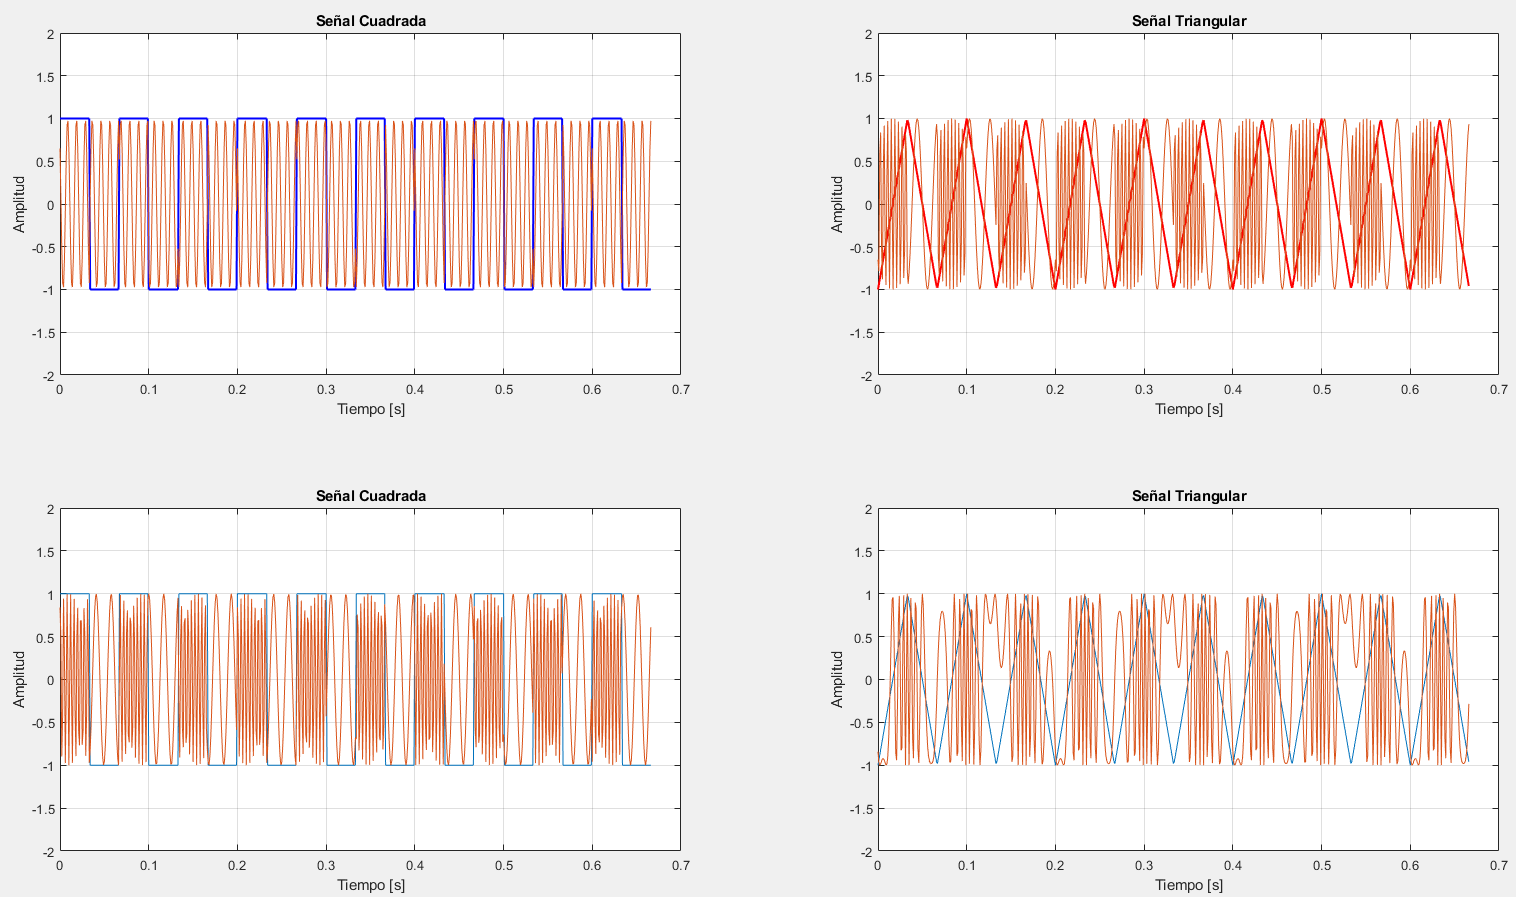
\includegraphics[width=0.5\textwidth]{media/relacion_pm_fm}
		\caption{Diferencias y relaciones entre la modulación FM y PM}
		\label{fig:relacionpmfm}
	\end{figure}
	
	De este análisis se puede destacar que una señal FM aunque más común resulta un proceso más caro debido a que requiere una mayor cantidad de componentes para su implementación, sin embargo sus beneficios como su alta inmunidad al ruido la convirtieron en un método ideal para la transmisión de radio.
	
	\bibliographystyle{IEEEtran}
	\bibliography{biblio}
\end{document}
